\documentclass{beamer}
%
% Choose how your presentation looks.
%
% For more themes, color themes and font themes, see:
% http://deic.uab.es/~iblanes/beamer_gallery/index_by_theme.html
%
\mode<presentation>
{
  \usetheme{default}      % or try Darmstadt, Madrid, Warsaw, ...
  \usecolortheme{default} % or try albatross, beaver, crane, ...
  \usefonttheme{default}  % or try serif, structurebold, ...
  \setbeamertemplate{navigation symbols}{}
  \setbeamertemplate{caption}[numbered]
} 

\usepackage[english]{babel}
\usepackage[utf8x]{inputenc}

\title[Text to Image Synthesis]{Text to Image Synthesis}
\author{Andrew Drozdov}
\institute{NYU Department of Computer Science}
\date{August 8, 2017}

\begin{document}

\begin{frame}
  \titlepage
\end{frame}

% Uncomment these lines for an automatically generated outline.
%\begin{frame}{Outline}
%  \tableofcontents
%\end{frame}


%%%%%%%%%%%%%%
% Section: Overview   %
%%%%%%%%%%%%%%
\section{Overview}
\begin{frame}{}
\centering
Overview
\end{frame}


% TODO: Maybe want to cover image-to-text first?
% Summary Header
\begin{frame}{Paper Summary: Reed et al., 2016}
\centering
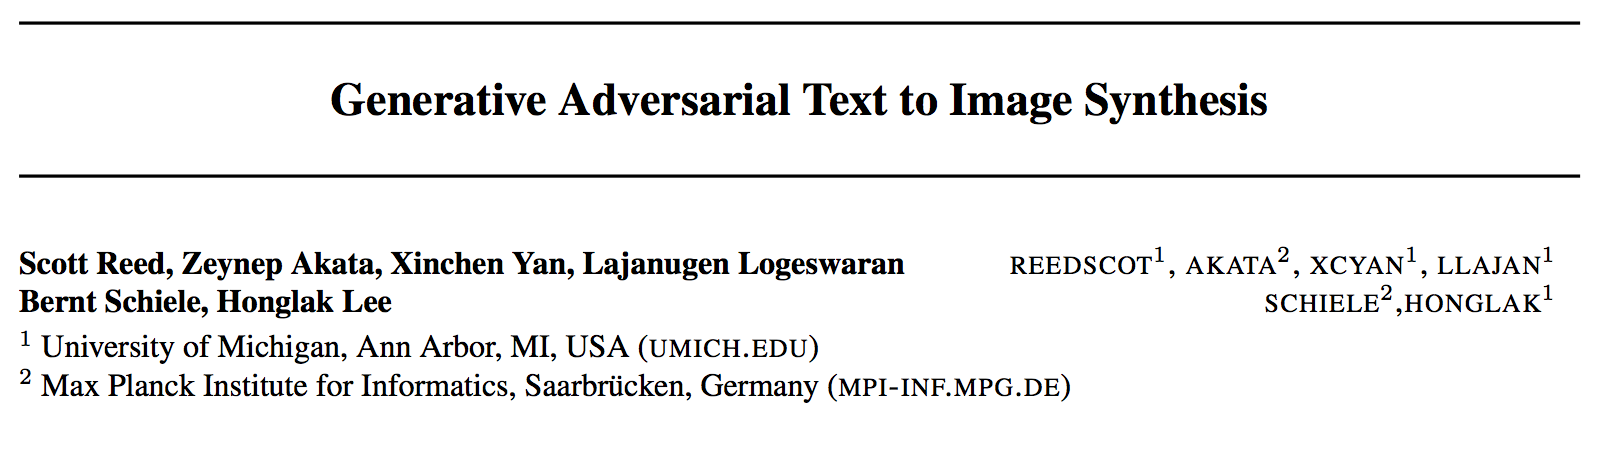
\includegraphics[width=10cm]{img/reed/header.png}
\vskip 0.1cm
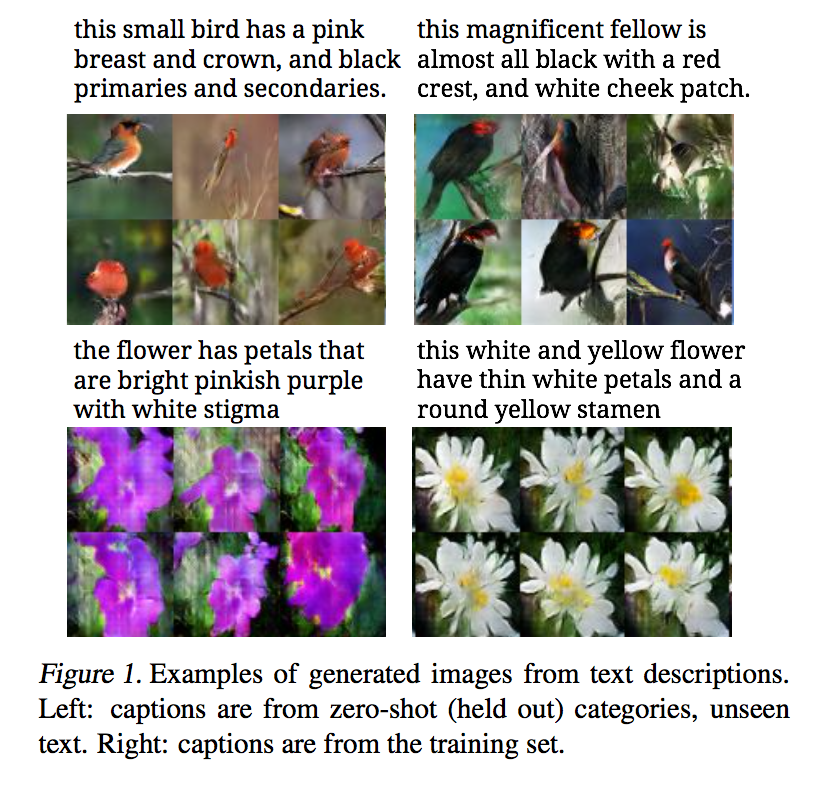
\includegraphics[width=5cm]{img/reed/figure1.png}
\end{frame}


% What is the meaning of meaning?
\begin{frame}{What is the problem?}
\centering
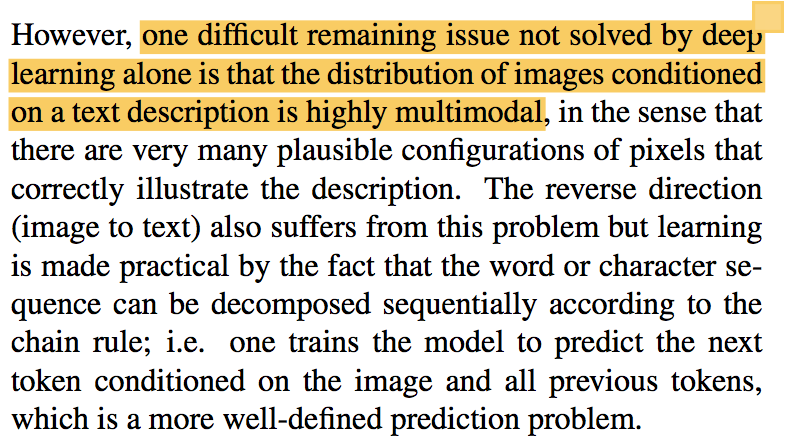
\includegraphics[width=10cm]{img/reed/problem.png}
\end{frame}


%%%%%%%%%%%%%%
% Section: Background   %
%%%%%%%%%%%%%%
\section{Background}
\begin{frame}{}
\centering
Background
\end{frame}


% What is the solution?
\begin{frame}{Generative Adversarial Networks (Goodfellow et al. 2014)}
Play this minimax game until reaching a Nash equilibrium:
\vskip0.5cm
\centering
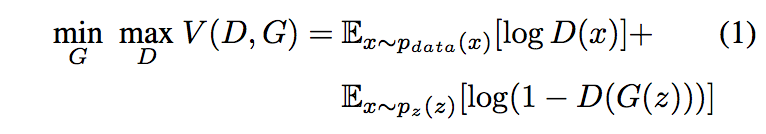
\includegraphics[width=10cm]{img/reed/gan_eq.png}

\begin{minipage}{0.48\textwidth}
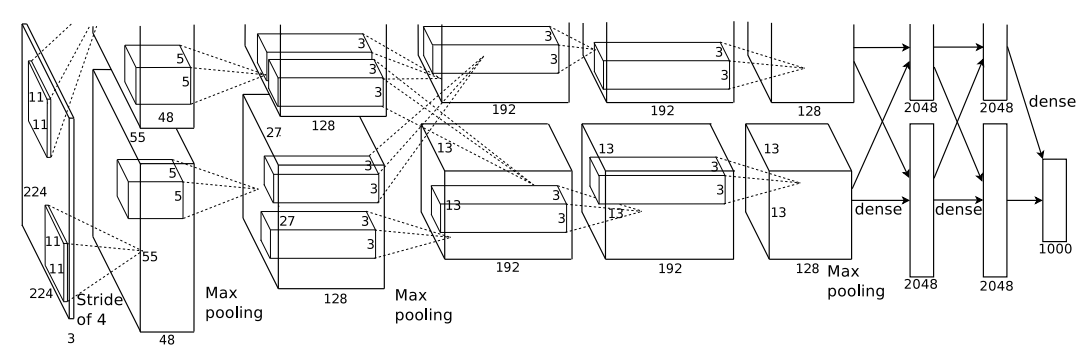
\includegraphics[width=1.0\linewidth]{img/reed/imagenet_cnn.png}
\end{minipage}
(Krizhevsky et al. 2012)
\hfill
\begin{minipage}{0.48\textwidth}
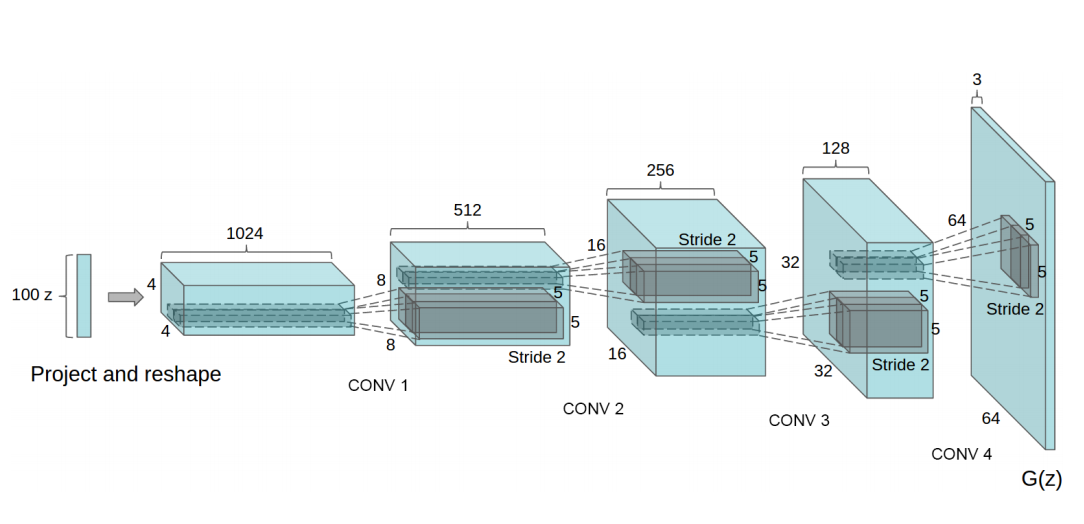
\includegraphics[width=1.0\linewidth]{img/reed/dcgan.png}
\end{minipage}
(Radford et al. 2015)

\end{frame}


% TODO: Compare to Karpathy approach (or to Elman approach)?
% What is a CNN+RNN?
\begin{frame}{Joint Embedding (Reed et al. 2016)}

\begin{center}
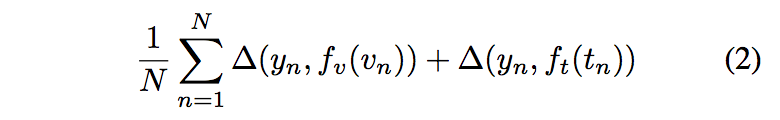
\includegraphics[width=10cm]{img/reed/joint.png}
\end{center}

\begin{itemize}
\item $v_n$ - image
\item $y_n$ - image class
\item $t_n$ - image description
\end{itemize}

\begin{center}
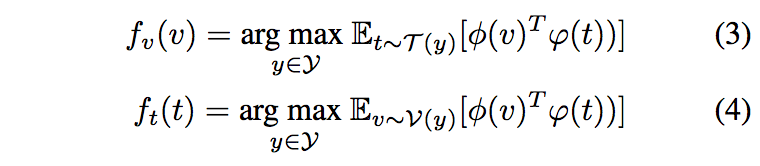
\includegraphics[width=10cm]{img/reed/classifiers.png}
\end{center}

\begin{itemize}
\item $\phi$ - image encoder
\item $\psi$ - text encoder
\item $f_v$ - image classifier
\item $f_t$ - text classifier

\end{itemize}
\end{frame}


%%%%%%%%%%%%%
% Section: Method  %
%%%%%%%%%%%%%
\section{Method}
\begin{frame}{}
\centering
Method
\end{frame}


% Model
\begin{frame}{Model}

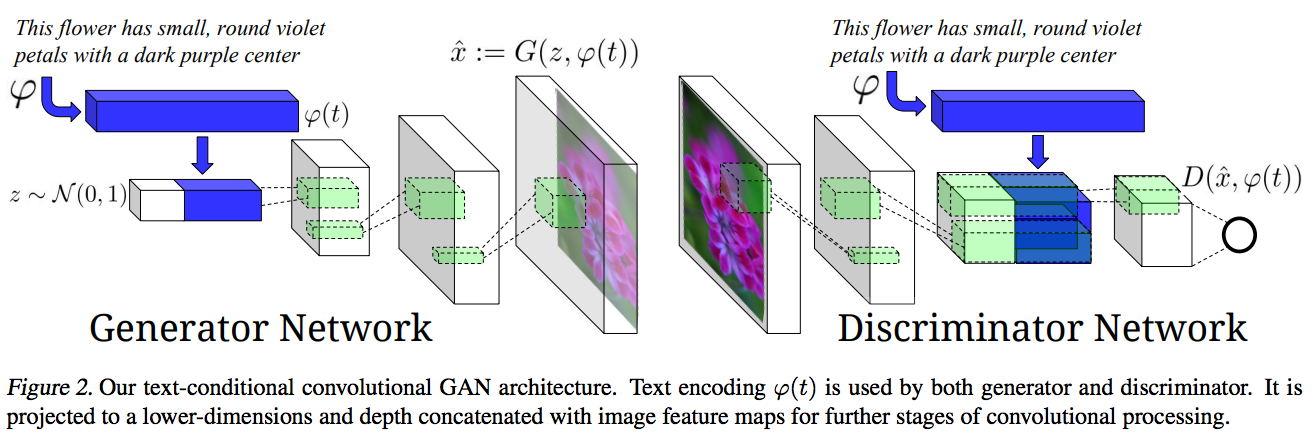
\includegraphics[width=1.0\linewidth]{img/reed/model.png}

\end{frame}


% Joint Conditioning Problem
\begin{frame}{Joint Conditioning of Image and Description (GAN-CLS)}
Easily discriminate early in training but later...
\vskip 0.5cm

What we have:
\begin{itemize}
\item Real Image + Matching Description
\item Fake Image + Arbitrary Description (Matching or Not Matching)
\end{itemize}
\vskip 0.5cm

What we may need:
\begin{itemize}
\item Real Image + Not Matching Description (Learn to match)
\end{itemize}
\end{frame}


% Embedding Interpolation
\begin{frame}{Data Augmentation by Interpolation (GAN-INT)}
Create additional \textit{text embeddings} (using interpolation between existing embeddings).
\vskip 0.5cm

Assumption: ``interpolations between embedding pairs tend to be near the data manifold'' (Bengio et al., 2013; Reed et al., 2014)
\vskip 0.5cm

\centering
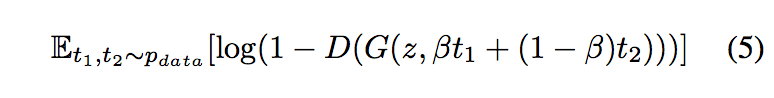
\includegraphics[width=10cm]{img/reed/interpolation.png}

\end{frame}


% Style Transfer
\begin{frame}{Style Transfer}
The text encodes the content; the image encodes the style. \\
The text is easy to manipulate; the image not so.
\vskip 0.5cm

\begin{block}{Convolutional Style Network:}
$$S: R^D \rightarrow R^Z$$
\end{block}
\vskip 0.5cm

\begin{block}{Style Loss:}
\centering
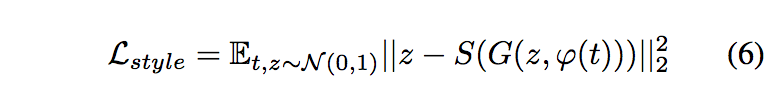
\includegraphics[width=10cm]{img/reed/style_loss.png}
\end{block}
\vskip 0.5cm

\begin{block}{Style Transfer:}
\centering

\includegraphics[width=10cm]{img/reed/style_transfer.png}
\end{block}

\end{frame}


%%%%%%%%%%%%%
% Section: Results   %
%%%%%%%%%%%%%
\section{Results}
\begin{frame}{}
\centering
Results
\end{frame}


% Data
\begin{frame}{Datasets}

\begin{itemize} % start
\item Birds - CUB dataset
\begin{itemize}
\item 11,788 images
\item 200 categories
\item 150 train+val classes
\item 50 test classes
\end{itemize}

\item Flowers - Oxford-102 dataset
\begin{itemize}
\item 8,189 images
\item 102 categories
\item 82 train+val classes
\item 20 test classes
\end{itemize}

\item 5 captions per image
\item Augment images with random transformation: scale, crop, etc.

\end{itemize} % end

\end{frame}


% Model Summary
\begin{frame}{Model Summary}
\begin{itemize}
\item GAN
\item GAN-CLS (real image, fake label)
\item GAN-INT (text interpolation)
\item GAN-INT-CLS
\item Style Transfer
\end{itemize}
\end{frame}


% Zero-Shot Birds
\begin{frame}{Zero Shot: Birds}
\centering
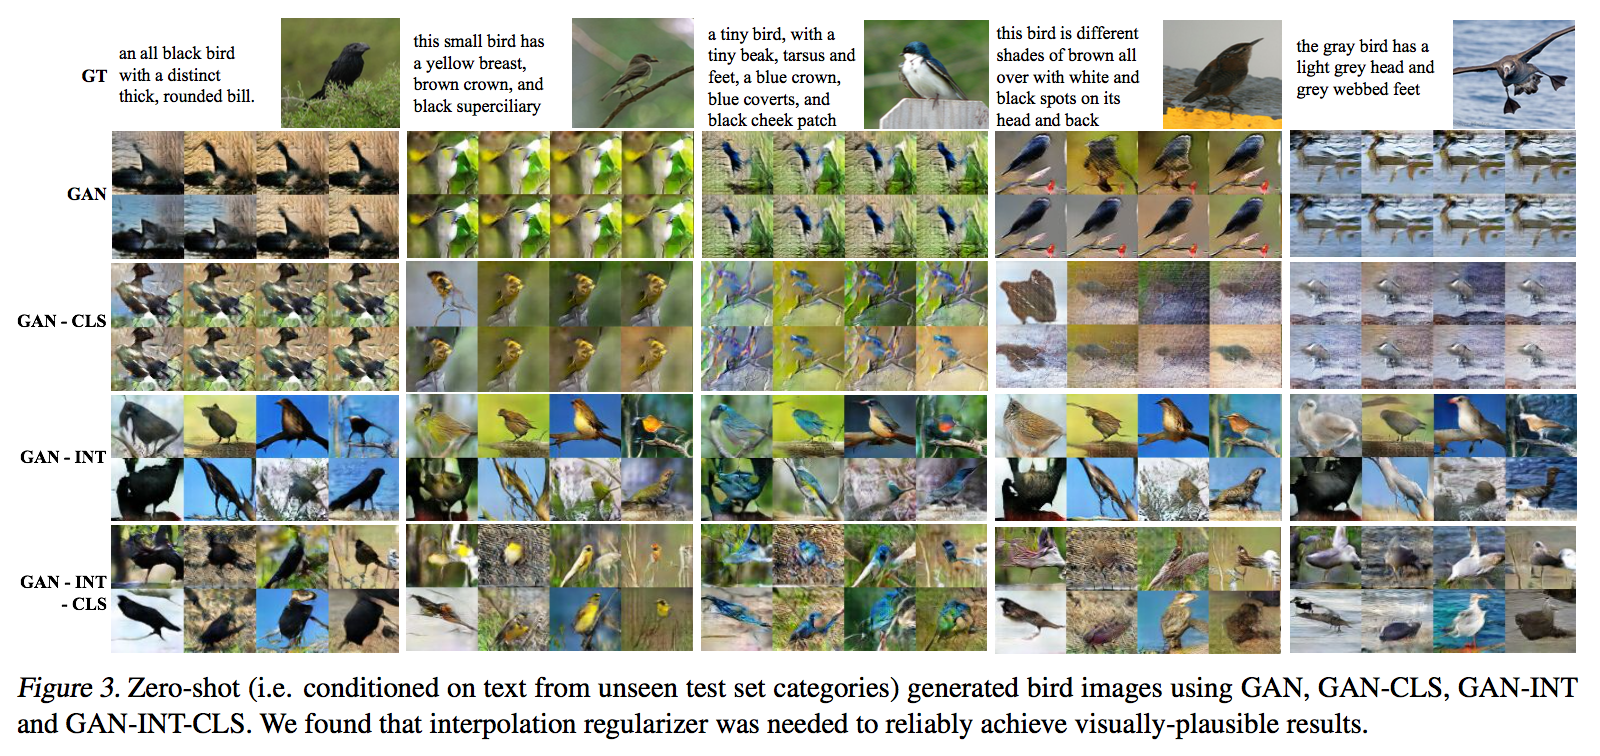
\includegraphics[width=10cm]{img/reed/zero_shot_birds.png}
\end{frame}


% Zero-Shot Flowers
\begin{frame}{Zero Shot: Flowers}
\centering
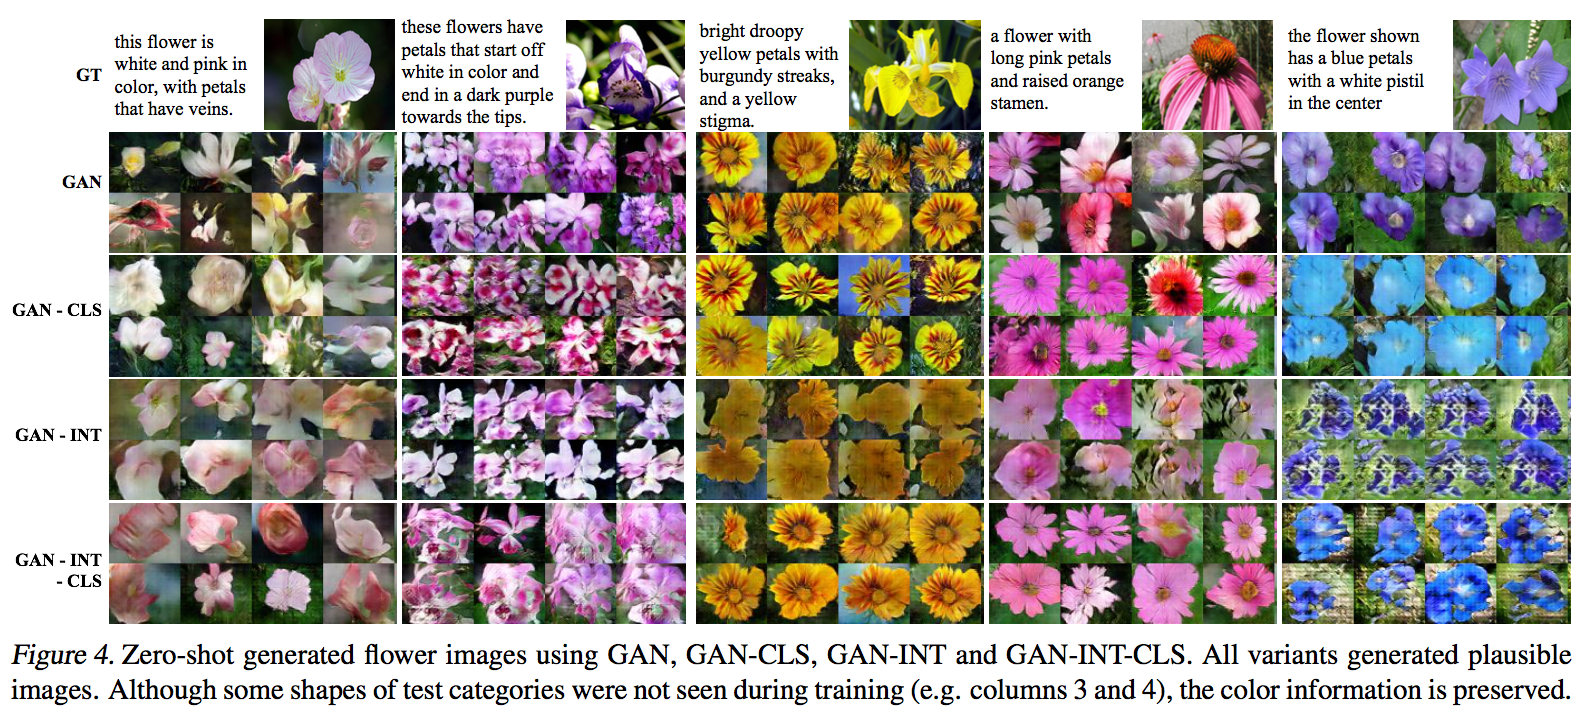
\includegraphics[width=10cm]{img/reed/zero_shot_flowers.png}
\end{frame}


% Style Transfer
\begin{frame}{Style Transfer: Birds}
\begin{itemize}
\item 100 Clusters (K-means)
\item Background: RGB
\item Pose: 6 keypoint coordinates (beak, belly, breast, crown, forehead, and tail)
\end{itemize}

\centering
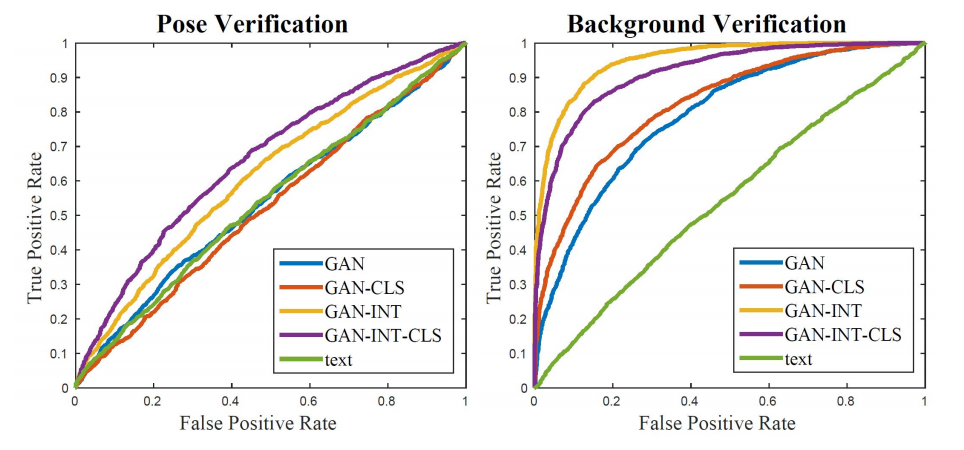
\includegraphics[width=1.0\linewidth]{img/reed/style_roc.png}
\end{frame}


% Style Transfer
\begin{frame}{Style Transfer: Birds}
\centering
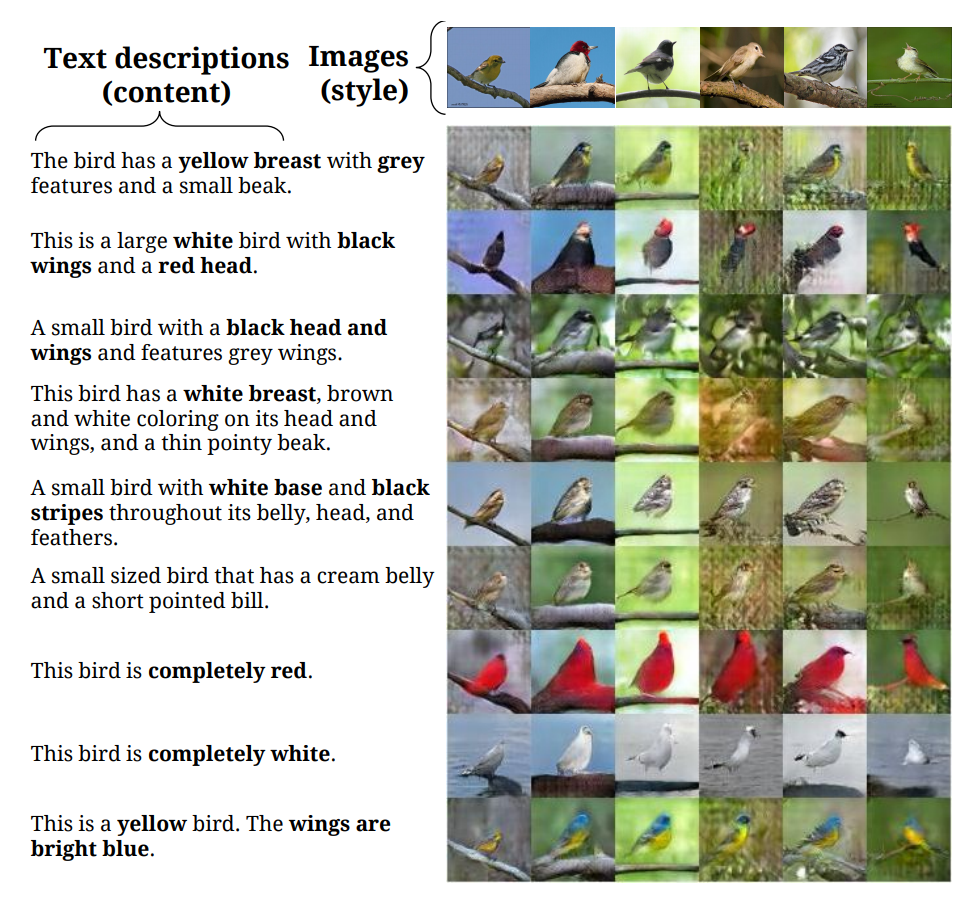
\includegraphics[width=9cm]{img/reed/style_examples.png}
\end{frame}


% Text Interpolation
\begin{frame}{Text Interpolation}
\centering
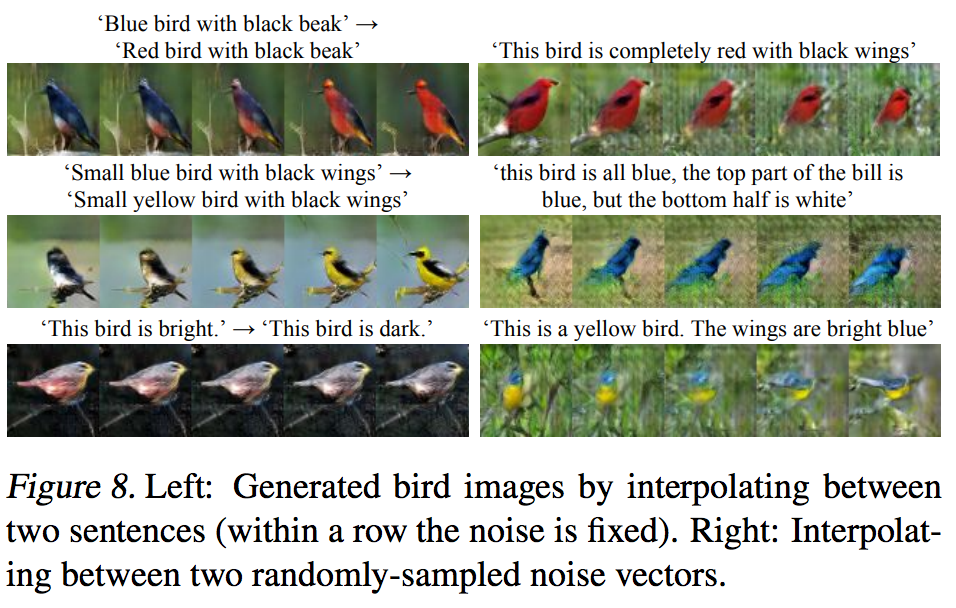
\includegraphics[width=9cm]{img/reed/result_text_int.png}
\end{frame}


% Beyond birds and flowers
\begin{frame}{Beyond birds and flowers}
\centering
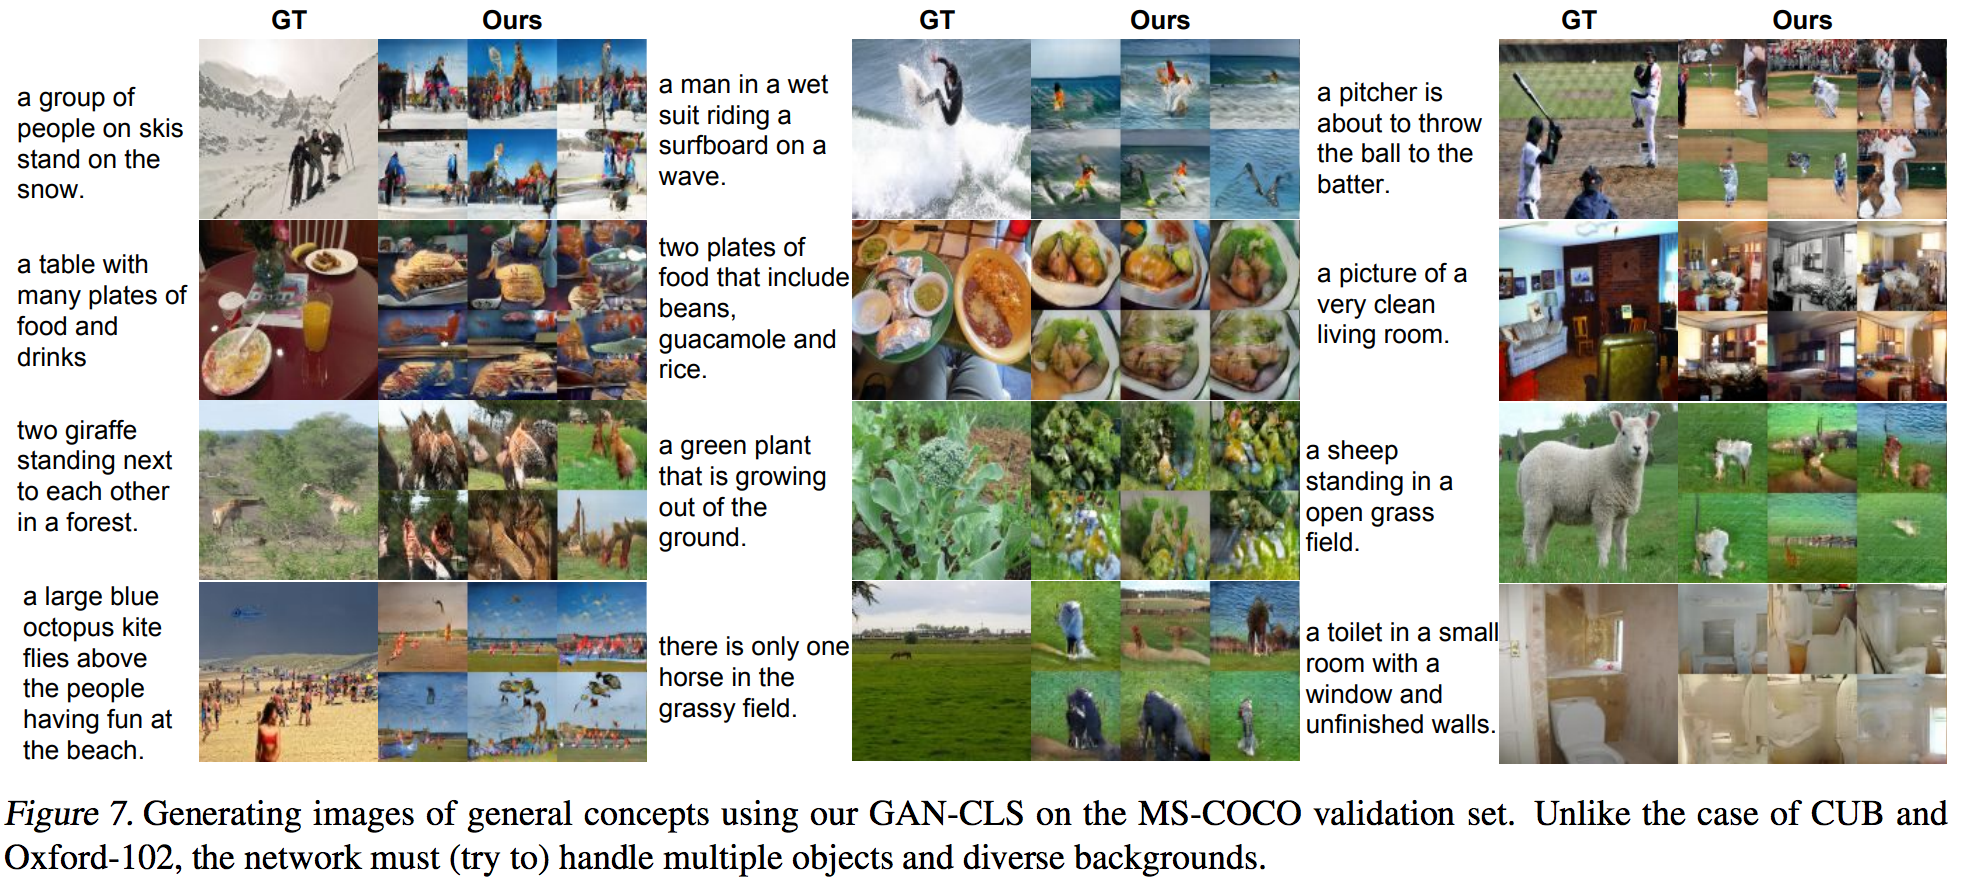
\includegraphics[width=9cm]{img/reed/result_beyond.png}
\end{frame}


%%%%%%%%%%%%%%%
% Section: Discussion   %
%%%%%%%%%%%%%%%
\section{Discussion}
\begin{frame}{}
\centering
Discussion
\end{frame}


% Question: What is an image from a text perspective?
\begin{frame}{Question for the Audience}
What is the closest representation to an image, in pure 100\% text?
\vskip 0.5cm

\begin{block}{Followup}
\begin{itemize}
\item Can we do text to image synthesis without $z$?
\item Can we do text to image synthesis with longer descriptions?
\item Can we do text to text synthesis (inverse summarization)?
\end{itemize}
\end{block}

\end{frame}


%%%%%%%%%%%%%%%
% Section: References   %
%%%%%%%%%%%%%%%
\section{References}
\begin{frame}{References}
\begin{enumerate}
\item[1] Goodfellow, Ian, Jean Pouget-Abadie, Mehdi Mirza, Bing Xu, David Warde-Farley, Sherjil Ozair, Aaron Courville, and Yoshua Bengio. "Generative adversarial nets." Advances in neural information processing systems. 2014.

\item[2] Krizhevsky, Alex, Ilya Sutskever, and Geoffrey E. Hinton. "Imagenet classification with deep convolutional neural networks." Advances in neural information processing systems. 2012.

\item[3] Radford, Alec, Luke Metz, and Soumith Chintala. "Unsupervised representation learning with deep convolutional generative adversarial networks." arXiv preprint arXiv:1511.06434 (2015). (ICLR 2016)
\end{enumerate}
\end{frame}

%
\begin{frame}{References}
\begin{enumerate}
\item[4] Reed, S., Akata, Z., Lee, H., and Schiele, B. Learning deep representations for fine-grained visual descriptions. In CVPR, 2016.

\item[5] Gauthier, J. Conditional generative adversarial nets for convolutional face generation. Technical report, 2015.

\item[6] Bengio, Y., Mesnil, G., Dauphin, Y., and Rifai, S. Better mixing via deep representations. In ICML, 2013.
\end{enumerate}
\end{frame}

%
\begin{frame}{References}
\begin{enumerate}
\item[7] Reed, S., Akata, Z., Lee, H., and Schiele, B. Learning deep representations for fine-grained visual descriptions. In CVPR, 2016.

\item[8] Reed, S., Sohn, K., Zhang, Y., and Lee, H. Learning to disentangle factors of variation with manifold interaction. In ICML, 2014.
\end{enumerate}
\end{frame}



\end{document}
